\begin{comment}
\documentclass[10pt]{article}
\usepackage{fullpage, graphicx, url}
\setlength{\parskip}{1ex}
\setlength{\parindent}{0ex}
\title{rnd31}
\begin{document}


\begin{tabular}{ccc}
The Alternative Csound Reference Manual & & \\
Previous & &Next

\end{tabular}

%\hline 
\end{comment}
\section{rnd31}
rnd31�--� 31-bit bipolar random opcodes with controllable distribution. \subsection*{Description}


  31-bit bipolar random opcodes with controllable distribution. These units are portable, i.e. using the same seed value will generate the same random sequence on all systems. The distribution of generated random numbers can be varied at k-rate. 
\subsection*{Syntax}


 ax \textbf{rnd31}
 kscl, krpow [, iseed]


 ix \textbf{rnd31}
 iscl, irpow [, iseed]


 kx \textbf{rnd31}
 kscl, krpow [, iseed]
\subsection*{Initialization}


 \emph{ix}
 -- i-rate output value. 


 \emph{iscl}
 -- output scale. The generated random numbers are in the range -iscl to iscl. 


 \emph{irpow}
 -- controls the distribution of random numbers. If irpow is positive, the random distribution (x is in the range -1 to 1) is \emph{abs(x) \^{} ((1 / irpow) - 1)}
; for negative irpow values, it is \emph{(1 - abs(x)) \^{} ((-1 / irpow) - 1)}
. Setting \emph{irpow}
 to -1, 0, or 1 will result in uniform distribution (this is also faster to calculate). 


 


 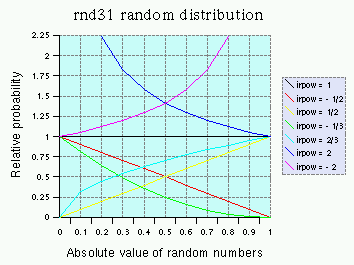
\includegraphics[scale=1]{rnd31_rand} 


 A graph of distributions for different values of irpow.


 \emph{iseed}
 (optional, default=0) -- seed value for random number generator (positive integer in the range 1 to 2147483646 (2 \^{} 31 - 2)). Zero or negative value seeds from current time (this is also the default). Seeding from current time is guaranteed to generate different random sequences, even if multiple random opcodes are called in a very short time. 


  In the a- and k-rate version the seed is set at opcode initialization. With i-rate output, if iseed is zero or negative, it will seed from current time in the first call, and return the next value from the random sequence in successive calls; positive seed values are set at all i-rate calls. The seed is local for a- and k-rate, and global for i-rate units. 


 


\begin{tabular}{cc}
\textbf{Notes}
 \\
� &

 


 
\begin{itemize}
\item 

 although seed values up to 2147483646 are allowed, it is recommended to use smaller numbers ($<$ 1000000) for portability, as large integers may be rounded to a different value if 32-bit floats are used.

\item 

 i-rate \emph{rnd31}
 with a positive seed will always produce the same output value (this is not a bug). To get different values, set seed to 0 in successive calls, which will return the next value from the random sequence.


\end{itemize}


\end{tabular}

\subsection*{Performance}


 \emph{ax}
 -- a-rate output value. 


 \emph{kx}
 -- k-rate output value. 


 \emph{kscl}
 -- output scale. The generated random numbers are in the range -kscl to kscl. It is the same as \emph{iscl}
, but can be varied at k-rate. 


 \emph{krpow}
 -- controls the distribution of random numbers. It is the same as \emph{irpow}
, but can be varied at k-rate. 
\subsection*{Examples}


  Here is an example of the rnd31 opcode at a-rate. It uses the files \emph{rnd31.orc}
 and \emph{rnd31.sco}
. 


 \textbf{Example 1. An example of the rnd31 opcode at a-rate.}

\begin{lstlisting}
/* rnd31.orc */
; Initialize the global variables.
sr = 44100
kr = 4410
ksmps = 10
nchnls = 1

; Instrument #1.
instr 1
  ; Create random numbers at a-rate in the range -2 to 2 with 
  ; a triangular distribution, seed from the current time.
  a31 rnd31 2, -0.5

  ; Use the random numbers to choose a frequency.
  afreq = a31 * 500 + 100

  a1 oscil 30000, afreq, 1
  out a1
endin
/* rnd31.orc */
        
\end{lstlisting}
\begin{lstlisting}
/* rnd31.sco */
; Table #1, a sine wave.
f 1 0 16384 10 1

; Play Instrument #1 for one second.
i 1 0 1
e
/* rnd31.sco */
        
\end{lstlisting}


  Here is an example of the rnd31 opcode at k-rate. It uses the files \emph{rnd31\_krate.orc}
 and \emph{rnd31\_krate.sco}
. 


 \textbf{Example 2. An example of the rnd31 opcode at k-rate.}

\begin{lstlisting}
/* rnd31_krate.orc */
; Initialize the global variables.
sr = 44100
kr = 4410
ksmps = 10
nchnls = 1

; Instrument #1.
instr 1
  ; Create random numbers at k-rate in the range -1 to 1 
  ; with a uniform distribution, seed=10.
  k1 rnd31 1, 0, 10
        
  printks "k1=%f\\n", 0.1, k1
endin
/* rnd31_krate.orc */
        
\end{lstlisting}
\begin{lstlisting}
/* rnd31_krate.sco */
; Play Instrument #1 for one second.
i 1 0 1
e
/* rnd31_krate.sco */
        
\end{lstlisting}
 Its output should include lines like this: \begin{lstlisting}
k1=0.112106
k1=-0.274665
k1=0.403933
      
\end{lstlisting}


  Here is an example of the rnd31 opcode that uses the number 7 as a seed value. It uses the files \emph{rnd31\_seed7.orc}
 and \emph{rnd31\_seed7.sco}
. 


 \textbf{Example 3. An example of the rnd31 opcode that uses the number 7 as a seed value.}

\begin{lstlisting}
/* rnd31_seed7.orc */
; Initialize the global variables.
sr = 44100
kr = 4410
ksmps = 10
nchnls = 1

; Instrument #1.
instr 1
  ; i-rate random numbers with linear distribution, seed=7. 
  ; (Note that the seed was used only in the first call.)
  i1 rnd31 1, 0.5, 7
  i2 rnd31 1, 0.5
  i3 rnd31 1, 0.5
        
  print i1
  print i2
  print i3
endin
/* rnd31_seed7.orc */
        
\end{lstlisting}
\begin{lstlisting}
/* rnd31_seed7.sco */
; Play Instrument #1 for one second.
i 1 0 1
e
/* rnd31_seed7.sco */
        
\end{lstlisting}
 Its output should include lines like this: \begin{lstlisting}
instr 1:  i1 = -0.649
instr 1:  i2 = -0.761
instr 1:  i3 = 0.677
      
\end{lstlisting}


  Here is an example of the rnd31 opcode that uses the current time as a seed value. It uses the files \emph{rnd31\_time.orc}
 and \emph{rnd31\_time.sco}
. 


 \textbf{Example 4. An example of the rnd31 opcode that uses the current time as a seed value.}

\begin{lstlisting}
/* rnd31_time.orc */
; Initialize the global variables.
sr = 44100
kr = 4410
ksmps = 10
nchnls = 1

; Instrument #1.
instr 1
  ; i-rate random numbers with linear distribution,
  ; seeding from the current time. (Note that the seed 
  ; was used only in the first call.)
  i1 rnd31 1, 0.5, 0
  i2 rnd31 1, 0.5
  i3 rnd31 1, 0.5

  print i1
  print i2
  print i3
endin
/* rnd31_time.orc */
        
\end{lstlisting}
\begin{lstlisting}
/* rnd31_time.sco */
; Play Instrument #1 for one second.
i 1 0 1
e
/* rnd31_time.sco */
        
\end{lstlisting}
 Its output should include lines like this: \begin{lstlisting}
instr 1:  i1 = -0.691
instr 1:  i2 = -0.686
instr 1:  i3 = -0.358
      
\end{lstlisting}
\subsection*{Credits}


 Author: Istvan Varga


 New in version 4.16
%\hline 


\begin{comment}
\begin{tabular}{lcr}
Previous &Home &Next \\
rnd &Up &rspline

\end{tabular}


\end{document}
\end{comment}
